\documentclass{ctexart}
\usepackage[a4paper, margin=1in]{geometry}  % 设置边距
\usepackage{graphicx}  % 引入graphicx宏包
\usepackage{tikz}
\usetikzlibrary{calc}
\usetikzlibrary {backgrounds,through,intersections}
\usepackage{xcolor}

\begin{document}

    \begin{tikzpicture}
        \coordinate [label=left:\textcolor{blue}{$A$}] (A) at (0,0);
        \coordinate [label=right:\textcolor{blue}{$B$}] (B) at (1.25,0.25);
        \draw[blue] (A) -- (B);
    \end{tikzpicture}
   

    \begin{tikzpicture}
        \coordinate (A) at (0+0.1*rand,0+0.1*rand);
        \coordinate  (B) at (1.25+0.1*rand,0.25+0.1*rand);
        \draw[blue] (A) -- (B);
    \end{tikzpicture}

    \begin{tikzpicture}
        \coordinate (A) at ($ (0,0) + .1*(rand,rand) $);
        \coordinate  (B) at ($ (1.25,0.25) + .1*(rand,rand) $);
        \draw[blue] (A) -- (B);
    \end{tikzpicture}

    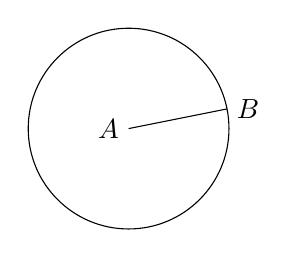
\begin{tikzpicture}
        \coordinate [label=left:$A$] (A) at (0,0);
        \coordinate [label=right:$B$] (B) at (1.25,0.25);
        \draw (A) -- (B);
        \draw (A) let
        \p1 = ($ (B) - (A) $)
        in
        circle ({veclen(\x1,\y1)});
    \end{tikzpicture}

    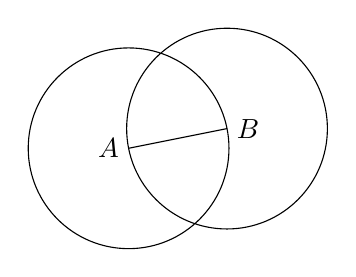
\begin{tikzpicture}
        \coordinate [label=left:$A$] (A) at (0,0);
        \coordinate [label=right:$B$] (B) at (1.25,0.25);
        \draw (A) -- (B);
        \draw let \p1 = ($ (B) - (A) $),
        \n2 = {veclen(\x1,\y1)}
        in
        (A) circle (\n2)
        (B) circle (\n2);
    \end{tikzpicture}

    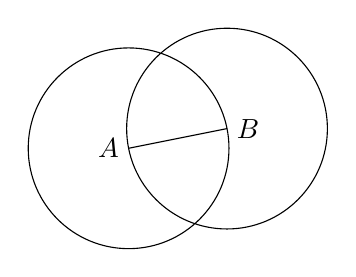
\begin{tikzpicture}
        \coordinate [label=left:$A$] (A) at (0,0);
        \coordinate [label=right:$B$] (B) at (1.25,0.25);
        \draw (A) -- (B);
        \draw let \p1 = ($ (B) - (A) $),
        \n2 = {veclen(\x1,\y1)}
        in
        (A) circle (\n2)
        (B) circle (\n2);
    \end{tikzpicture}

    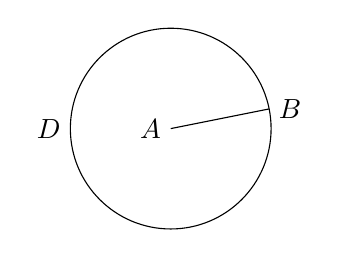
\begin{tikzpicture}
        \coordinate [label=left:$A$] (A) at (0,0);
        \coordinate [label=right:$B$] (B) at (1.25,0.25);
        \draw (A) -- (B);
        \node [draw,circle through=(B),label=left:$D$] at (A) {};
    \end{tikzpicture}

    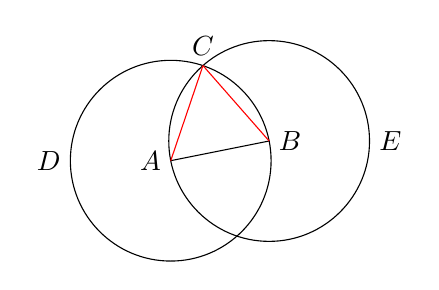
\begin{tikzpicture}
        \coordinate [label=left:$A$] (A) at (0,0);
        \coordinate [label=right:$B$] (B) at (1.25,0.25);
        \draw (A) -- (B);
        \node (D) [name path=D,draw,circle through=(B),label=left:$D$] at (A) {};
        \node (E) [name path=E,draw,circle through=(A),label=right:$E$] at (B) {};
        % Name the coordinates, but do not draw anything:
        \path [name intersections={of=D and E}];
        \coordinate [label=above:$C$] (C) at (intersection-1);
        \draw [red] (A) -- (C);
        \draw [red] (B) -- (C);
    \end{tikzpicture}

    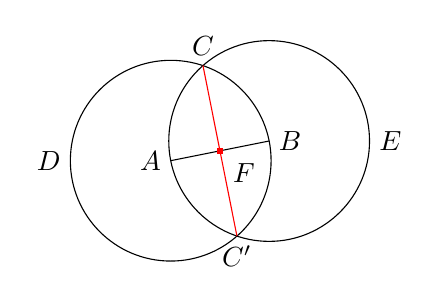
\begin{tikzpicture}
        \coordinate [label=left:$A$] (A) at (0,0);
        \coordinate [label=right:$B$] (B) at (1.25,0.25);
        \draw [name path=A--B] (A) -- (B);
        \node (D) [name path=D,draw,circle through=(B),label=left:$D$] at (A) {};
        \node (E) [name path=E,draw,circle through=(A),label=right:$E$] at (B) {};

        \path [name intersections={of=D and E, by={[label=above:$C$]C, [label=below:$C'$]C'}}];
        \draw [name path=C--C',red] (C) -- (C');
        \path [name intersections={of=A--B and C--C',by=F}];
        \node [fill=red,inner sep=1pt,label=-45:$F$] at (F) {};
    \end{tikzpicture}

    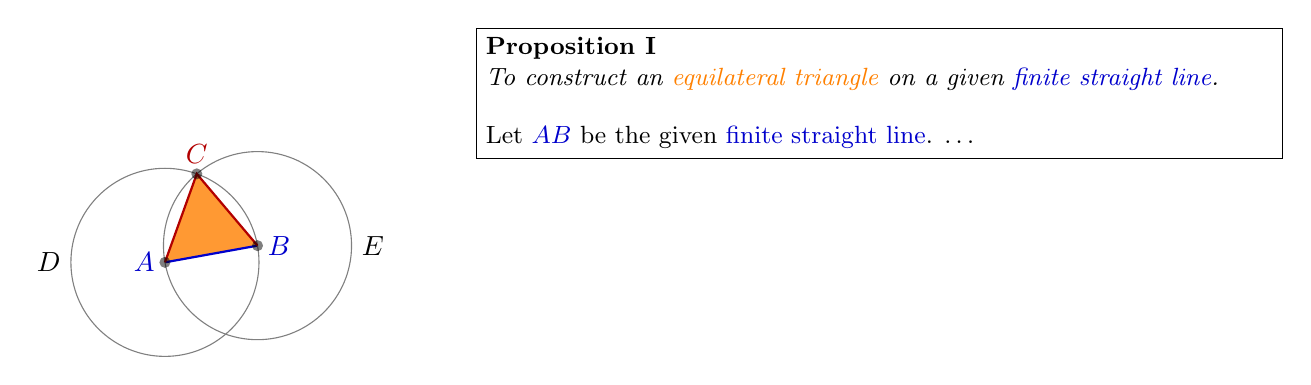
\begin{tikzpicture}[thick,help lines/.style={thin,draw=black!50}]
        \def\A{\textcolor{input}{$A$}} \def\B{\textcolor{input}{$B$}}
        \def\C{\textcolor{output}{$C$}} \def\D{$D$}
        \def\E{$E$}

        \colorlet{input}{blue!80!black} \colorlet{output}{red!70!black}
        \colorlet{triangle}{orange}


        \coordinate [label=left:\A] (A) at ($ (0,0) + .1*(rand,rand) $);
        \coordinate [label=right:\B] (B) at ($ (1.25,0.25) + .1*(rand,rand) $);

        \draw [input] (A) -- (B);

        \node [name path=D,help lines,draw,label=left:\D] (D) at (A) [circle through=(B)] {};
        \node [name path=E,help lines,draw,label=right:\E] (E) at (B) [circle through=(A)] {};

        \path [name intersections={of=D and E,by={[label=above:\C]C}}];
        \draw [output] (A) -- (C) -- (B);
        \foreach \point in {A,B,C}
            \fill [black,opacity=.5] (\point) circle (2pt);

        \begin{pgfonlayer}{background}
            \fill[triangle!80] (A) -- (C) -- (B) -- cycle;
        \end{pgfonlayer}

        \node [ draw,below right,text width=10cm,align=justify] at (4,3) {
            \small\textbf{Proposition I}\par
            \emph{To construct an \textcolor{triangle}{equilateral triangle}
            on a given \textcolor{input}{finite straight line}.}
            \par\vskip1em
            Let \A\B\ be the given \textcolor{input}{finite straight line}. \dots
        } ;
    \end{tikzpicture}

    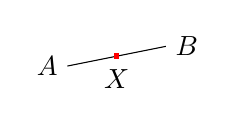
\begin{tikzpicture}
        \coordinate [label=left:$A$] (A) at (0,0);
        \coordinate [label=right:$B$] (B) at (1.25,0.25);
        \draw (A) -- (B);
        \node [fill=red,inner sep=1pt,label=below:$X$] (X) at ($ (A)!.5!(B) $) {};
    \end{tikzpicture}

    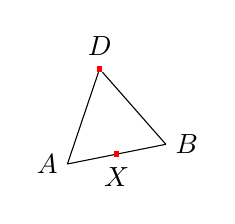
\begin{tikzpicture}
        \coordinate [label=left:$A$] (A) at (0,0);
        \coordinate [label=right:$B$] (B) at (1.25,0.25);
        \draw (A) -- (B);
        \node [fill=red,inner sep=1pt,label=below:$X$] (X) at ($ (A)!.5!(B) $) {};
        \node [fill=red,inner sep=1pt,label=above:$D$] (D) at
        ($ (X) ! {sin(60)*2} ! 90:(B) $) {};
        \draw (A) -- (D) -- (B);
    \end{tikzpicture}

    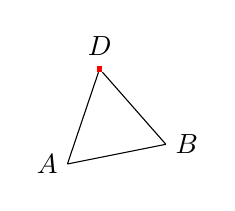
\begin{tikzpicture}
        \coordinate [label=left:$A$] (A) at (0,0);
        \coordinate [label=right:$B$] (B) at (1.25,0.25);
        \draw (A) -- (B);
        \node [fill=red,inner sep=1pt,label=above:$D$] (D) at
        ($ (A) ! .5 ! (B) ! {sin(60)*2} ! 90:(B) $) {};
        \draw (A) -- (D) -- (B);
    \end{tikzpicture}
    
    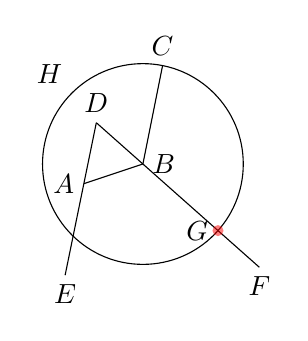
\begin{tikzpicture}
        \coordinate [label=left:$A$] (A) at (0,0);
        \coordinate [label=right:$B$] (B) at (0.75,0.25);
        \coordinate [label=above:$C$] (C) at (1,1.5);
        \draw (A) -- (B) -- (C);
        \coordinate [label=above:$D$] (D) at
        ($ (A) ! .5 ! (B) ! {sin(60)*2} ! 90:(B) $) {};
        \node (H) [label=135:$H$,draw,circle through=(C)] at (B) {};
        \draw (D) -- ($ (D) ! 3.5 ! (B) $) coordinate [label=below:$F$] (F);
        \draw (D) -- ($ (D) ! 2.5 ! (A) $) coordinate [label=below:$E$] (E);
        \path let \p1 = ($ (B) - (C) $) in
            coordinate [label=left:$G$] (G) at ($ (B) ! veclen(\x1,\y1) ! (F) $);
        \fill[red,opacity=.5] (G) circle (2pt);
    \end{tikzpicture}

    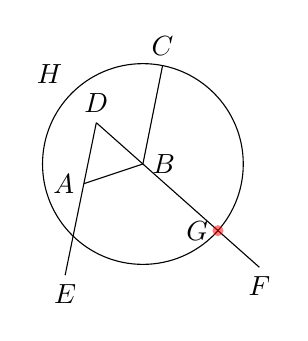
\begin{tikzpicture}
        \coordinate [label=left:$A$] (A) at (0,0);
        \coordinate [label=right:$B$] (B) at (0.75,0.25);
        \coordinate [label=above:$C$] (C) at (1,1.5);
        \draw (A) -- (B) -- (C);
        \coordinate [label=above:$D$] (D) at
        ($ (A) ! .5 ! (B) ! {sin(60)*2} ! 90:(B) $) {};
        \node (H) [name path=H,label=135:$H$,draw,circle through=(C)] at (B) {};
        \draw (D) -- ($ (D) ! 3.5 ! (B) $) coordinate [label=below:$F$] (F);
        \draw (D) -- ($ (D) ! 2.5 ! (A) $) coordinate [label=below:$E$] (E);
        \path [name path=B--F] (B) -- (F);
        \path [name intersections={of=H and B--F,by={[label=left:$G$]G}}];
        \fill[red,opacity=.5] (G) circle (2pt);
    \end{tikzpicture}

    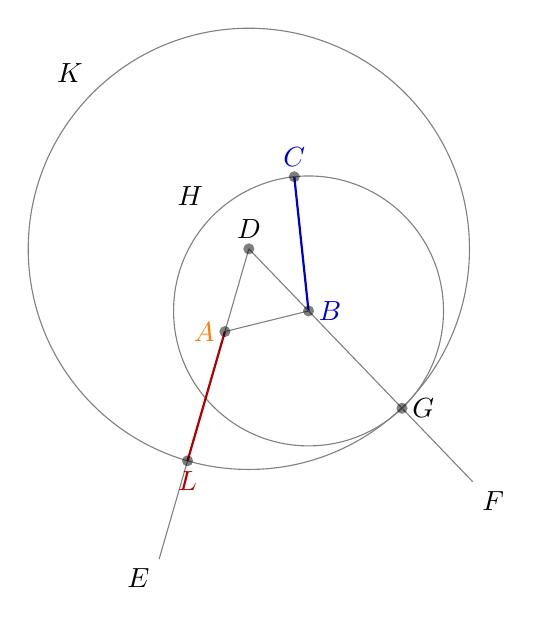
\begin{tikzpicture}[thick,help lines/.style={thin,draw=black!50}]
        \def\A{\textcolor{orange}{$A$}} \def\B{\textcolor{input}{$B$}}
        \def\C{\textcolor{input}{$C$}} \def\D{$D$}
        \def\E{$E$} \def\F{$F$}
        \def\G{$G$} \def\H{$H$}
        \def\K{$K$} \def\L{\textcolor{output}{$L$}}

        \colorlet{input}{blue!80!black} \colorlet{output}{red!70!black}

        \coordinate [label=left:\A] (A) at ($ (0,0) + .1*(rand,rand) $);
        \coordinate [label=right:\B] (B) at ($ (1,0.2) + .1*(rand,rand) $);
        \coordinate [label=above:\C] (C) at ($ (1,2) + .1*(rand,rand) $);

        \draw [input] (B) -- (C);
        \draw [help lines] (A) -- (B);

        \coordinate [label=above:\D] (D) at ($ (A)!.5!(B) ! {sin(60)*2} ! 90:(B) $);
        \draw [help lines] (D) -- ($ (D)!3.75!(A) $) coordinate [label=-135:\E] (E);
        \draw [help lines] (D) -- ($ (D)!3.75!(B) $) coordinate [label=-45:\F] (F);

        \node (H) at (B) [name path=H,help lines,circle through=(C),draw,label=135:\H] {};
        \path [name path=B--F] (B) -- (F);
        \path [name intersections={of=H and B--F,by={[label=right:\G]G}}];

        \node (K) at (D) [name path=K,help lines,circle through=(G),draw,label=135:\K] {};
        \path [name path=A--E] (A) -- (E);
        \path [name intersections={of=K and A--E,by={[label=below:\L]L}}];

        \draw [output] (A) -- (L);

        \foreach \point in {A,B,C,D,G,L}
            \fill [black,opacity=.5] (\point) circle (2pt);
    \end{tikzpicture}
\end{document}